\documentclass[border=0.8ex,svgnames,tikz]{standalone}
\usepackage{amsmath,mathtools}
\usepackage{fontspec}
\setmainfont{Source Serif 4}
\setsansfont{Source Sans 3}
\setmonofont{Source Code Pro}
\begin{document}
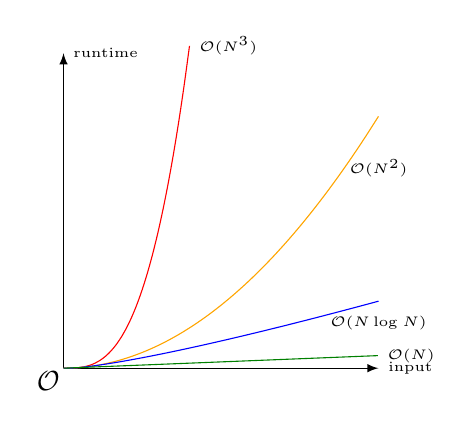
\begin{tikzpicture}
  \path[draw,->,>=latex] (0,0) --  (4,0) node[right,font=\tiny]{input};
  \path[draw,->,>=latex] (0,0) --  (0,4) node[right,font=\tiny]{runtime};
  \node[below left=-0.5ex] at (0,0) {$\mathcal{O}$};
  \path[draw=Red,smooth,domain=0.001:8,xscale=0.2,yscale=0.008] plot
  (\x,\x*\x*\x) node[right] {\tiny $\mathcal{O}(N^{3})$};
  \path[draw=Orange,smooth,domain=0.001:20,xscale=0.2,yscale=0.008] plot
  (\x,\x*\x) node[below=12] {\tiny $\mathcal{O}(N^{2})$};
  \path[draw=Blue,smooth,domain=0.001:40,xscale=0.1,yscale=0.004]
  plot(\x,{\x*log2(\x)}) node[below=2] {\tiny $\mathcal{O}(N \log_{}{N})$};
  \path[draw=Green,smooth,domain=0.0000001:0.04,xscale=100,yscale=4] plot
  (\x,{\x}) node[right] {\tiny $\mathcal{O}(N)$};
\end{tikzpicture}
\end{document}
